\documentclass[a4paper, 10pt]{article}%тип документа

%Русский язык
\usepackage[T2A]{fontenc} %кодировка
\usepackage[utf8]{inputenc} %кодировка исходного кода
\usepackage[english,russian]{babel} %локализация и переносы

%Вставка картинок
\usepackage{graphicx}
\DeclareGraphicsExtensions{.pdf,.png,.jpg}

%Графики
\usepackage{pgfplots}
\pgfplotsset{compat=1.9}

%Математика
\usepackage{amsmath, amsfonts, amssymb, amsthm, mathtools}

%Заголовок
\author{Дербенев Никита Максимович}
\title{Определение систематических и случайных погрешностей при измерении удельного сопротивления нихромой проволоки \\
Лабораторная работа №1.1.1 по курсу Общая физика}
\date{7 сентября 2023}
\begin{document}
\maketitle 
\newpage
В работе используеются: линейка, линейка, штангенциркуль, микрометр, отрезок проволоки из нихрома, амперметр, вольтметр, источник ЭДС, мост постоянного тока, реостат, ключ. 
\begin{enumerate}
\item Точность измерения с помощью штангенциркуля -- 0,1 мм. Точность измерения с помощью микрометра -- 0,01 мм.
\item Измеряем диаметр проволки с помощью штангенциркуля ($d_1$, табл. 1) и микрометра ($d_2$, табл. 2) на 10 различных участках (табл. 1) \\
\begin{table}[h]
\caption{Результаты измерения диаметра проволоки}
\centering
\begin{tabular}{|r|c|c|c|c|c|c|c|c|c|c|c|}
\hline
& 1 & 2 & 3 & 4 & 5 & 6 & 7 & 8 & 9 & 10\\
\hline
$d_1$, мм & 0.3 & 0.3 & 0.3 & 0.3 & 0.3 & 0.3 & 0.3 & 0.3 & 0.3 & 0.3 \\
\hline
$d_2$, мм & 0.37 & 0.38 & 0.37 & 0.36 & 0.36 & 0.36 & 0.36 & 0.38 & 0.36 & 0.35 \\
\hline
\multicolumn{1}{|r|}{} & \multicolumn{5}{c}{ \( \overline{d_{1}} = 0.3 мм \) мм}  & \multicolumn{5}{c|}{ \( \overline{d_{2}} = 0.365 мм \) мм}\\
\hline
\end{tabular}
\end{table}

При измерении диаметра проволоки штангенциркулем случайная погрешность отсутствует. Следовательно, точность резульата определяется только точностью штангенциркуля (систематической погрешностью):
\begin{center}
\[ d_1 = (0.3 \pm 0.1) \text{ мм } \]
\end{center}

При измерении микрометром есть как систематичская, так и случайная ошибка:
\[ \sigma_{\text{сист}}  = 0.01 \text{ мм, }
\sigma_{\text{сл}}  = \dfrac{1}{N} \cdot \sqrt{\sum_{i = 1}^N (d - \overline{d})^2} = \frac{1}{10}\sqrt{8.5\cdot10^{-4}} \approx 2.915\cdot10^{-4} \text{ мм}\]
\[ \sigma =  \sqrt{\sigma_{\text{сист}}^2 + \sigma_{\text{сл}}^2} \approx 0.01 \text{мм}\]
Поскольку погрешность микрометра на порядок меньше погрешности штангенциркуля, для расчета площади поперечного сечения проволоки будем использовать значение, полученное измерением с помощью микрометра:
\[ d_2 = (0.365 \pm 0.1) \text{мм}\]
\item Определим площадь поперечного сечения проволоки: 
\[ S = \dfrac{ \pi d^2 }{4} = \dfrac{3,14 \cdot (0.365)^2}{4} \approx 0.105 \text{ мм}^2\]
Погрешность находим по формуле:
\[ \sigma_{s} = 2\dfrac{\sigma_{d_2}}{d_2}S = 2\dfrac{0.01}{0.365} \cdot 0.105 \text{ мм}^2 \approx 5.75 \cdot10^{-3} \text{ мм}^2 \]
Итак, $S = \left(0.105 \pm 0.006\right) \text{мм}^2$, то есть площадь определена с точностью 6\%.
\item Сведем основные хаактеристики приборов в таблицу (табл. 2) \\
\begin{table}[h]
\caption{Основные характеристики приборов при данном пределе}
\centering
\begin{tabular}{|p{3cm}|p{5cm}|p{5cm}|}
\hline
& Вольтметр & Миллиамперметр \\
\hline
Система & Электронная & Электромагнитная\\
\hline
Класс точности & 0.001 & 0.5 \\
\hline
Предел измерений $ x_{n} $ & 10 В & 300 мА \\
\hline
Число делений шкалы $n$ & 100000 & 150 \\
\hline
Цена делений $x_n / n$ & 0.1 мВ/дел & 2 мA/дел \\
\hline
Чувствительность $ n / x_n$ & 10000 дел/В & 500 дел/A \\
\hline
Абсолютная погрешность $\Delta x_M$ & 0.1мВ & 2 мА \\
\hline
Внутреннее сопротивление прибора & 10 МОм & 1 Ом\\
\hline
\end{tabular}
\end{table}

\item Очевидно, что надо мерять способом показанным на рис. 1a, так как погрешность измерений:

для схемы на рисунке 1а: $R_{\text{пр}}$/$R_{\text{V}} = 5\cdot10^{-7}$, т.е. около 0\%,

для схемы на рисунке 1б: $R_{\text{A}}$/$R_{\text{пр}} = 1/5 = 0.20$, т.е. 20\%.

\item Собираем схему рис. 1 \\
\begin{figure}[h]
\caption{Схема}
\centering
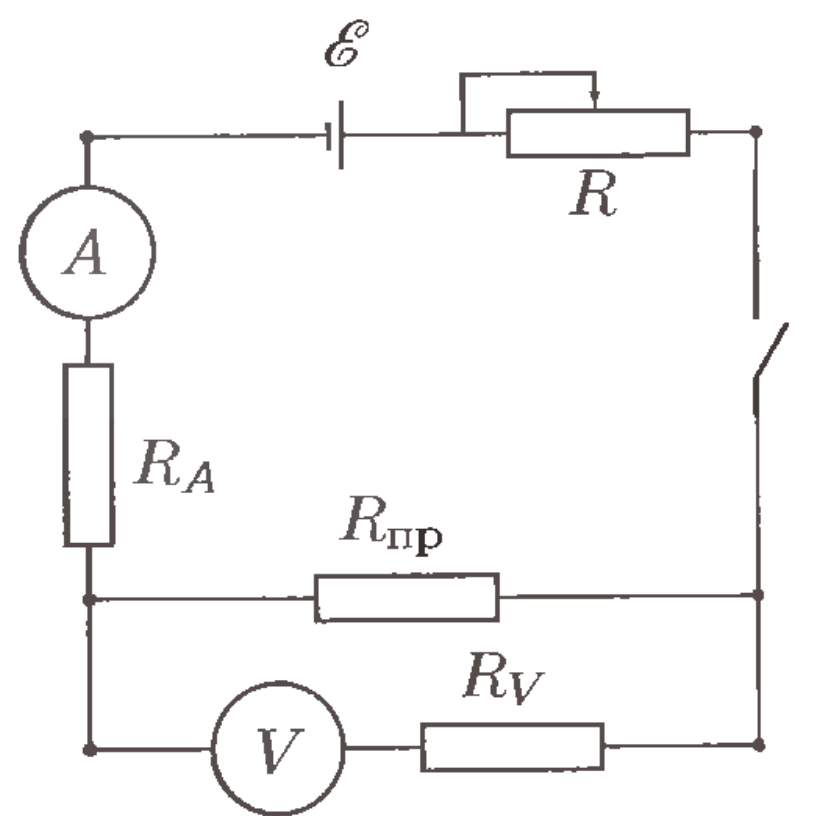
\includegraphics[scale=0.2]{sxema}
\end{figure}

\item Опыт проводим для трех длин проволоки: 
$ l_1 = (50\pm 0,1) \text{ см}, l_2 = (30\pm0,1) \text{ см}, l_3 = (20\pm 0,1) \text{ см.}$ \\
Измерения ведем для возрастающих и убывающих значений тока, все измерения записываем в табл. 3.
\begin{table}[h]
\caption{Показания приборов и результаты измерения сопротивления вольтметром, амперметром и при помощи моста}
\centering
\begin{tabular}{||c|c||c|c||c|c||c|c||}
\hline
\multicolumn{2}{||c||}{l = 20 см} & \multicolumn{2}{|c||}{l = 30 см} & \multicolumn{2}{|c||}{l = 50 см} \\
\hline
U, В & I, A & U, В & I, A & U, В & I, A \\
\hline
0.4202 & 0.198 & 0.6639 & 0.208 & 1.1322 & 0.216 \\
0.5047 & 0.238 & 0.7532 & 0.238 & 1.2426 & 0.236 \\
0.5438 & 0.256 & 0.8288 & 0.260 & 1.2885 & 0.246 \\
0.5732 & 0.270 & 0.9127 & 0.288 & 1.4783 & 0.282 \\
0.6138 & 0.290 & 0.9470 & 0.298 & 1.5814 & 0.301 \\
\hline
0.6010 & 0.284 & 0.9134 & 0.288 & 1.4153 & 0.270 \\
0.5839 & 0.275 & 0.8572 & 0.270 & 1.2968 & 0.247 \\
0.5525 & 0.260 & 0.8508 & 0.268 & 1.2818 & 0.244 \\
0.5080 & 0.240 & 0.7901 & 0.250 & 1.2007 & 0.227 \\
0.5044 & 0.238 & 0.7329 & 0.232 & 1.1598 & 0.221 \\
\hline
\multicolumn{2}{||c||}{$R_0$ = 2.133 Ом} & \multicolumn{2}{|c||}{$R_0$ = 3.1909 Ом} & \multicolumn{2}{|c||}{$R_0$ = 5.2679 Ом} \\
\multicolumn{2}{||c||}{$R_\text{ср}$ = 2.12 Ом} & \multicolumn{2}{|c||}{$R_\text{ср}$ = 3.17 Ом} & \multicolumn{2}{|c||}{$R_\text{ср}$ = 5.25 Ом} \\
\multicolumn{2}{||c||}{$\sigma_{R_\text{ср}}$ = 0.007} & \multicolumn{2}{|c||}{$\sigma_{R_\text{ср}}$ = 0.014} & \multicolumn{2}{|c||}{$\sigma_{R_\text{ср}}$ = 0.019} \\
\hline
\end{tabular}
\end{table}
\item Строим графики зависимостей U = f(I) для всех трех отрезков проволоки,  проводя прямые через экспериментальные точки (рис. 2). Из графиков видно, что нет различия между значениями, полученными при возрастании и уменьшении тока. Видно также, что случайный разброс точек пренебрежимо мал.
\begin{figure}[h]
\caption{График ВАХ для разных участков проволоки}
\centering
\begin{tikzpicture}
\begin{axis}[xlabel={I, А}, ylabel={U, В}, legend pos=south east]
\legend {20см,30см,50см}
\addplot[red,mark=x] coordinates {
(0,0)
(0.198,0.4202)
(0.238,0.5047)
(0.256,0.5438)
(0.270,0.5732)
(0.290,0.6138)
};
\addplot[green,mark=x] coordinates {
(0,0)
(0.208,0.6639)
(0.238,0.7532)
(0.260,0.8288)
(0.288,0.9127)
(0.298,0.9470)
};
\addplot[blue,mark=x] coordinates {
(0,0)
(0.216,1.1322)
(0.236,1.2426)
(0.246,1.2885)
(0.282,1.4783)
(0.301,1.5814)          
};
\addplot[red,mark=o] coordinates {
(0.284,0.6010)
(0.275,0.5839)
(0.260,0.5525)
(0.240,0.5080)
(0.238,0.5044)
(0,0)
};
\addplot[green,mark=o] coordinates {
(0.288,0.9134)
(0.270,0.8572)
(0.268,0.8508)
(0.250,0.7901)
(0.232,0.7329)    
(0,0)
};
\addplot[blue,mark=o] coordinates {
(0.270,1.4153)
(0.247,1.2968)
(0.244,1.2818)
(0.227,1.2007)
(0.221,1.1598)
(0,0)
};
\end{axis}
\end{tikzpicture}
\end{figure}
\item Для каждой длины l, используя график, находим среднее значение сопротивления по угловому коэффициенту соответствующей прямой: $R_\text{ср} = U/I$, где $U$ и $I$ - значение тока и напряжения, взятые на прямой в удобной точке у ее конца. Результаты запишем в табл. 3.
\item Погрешность $R_\text{ср}$ оцениваем по формуле \\
\[\dfrac{\sigma_{R_\text{ср}}}{R_\text{ср}} = \sqrt{\left(\dfrac{\sigma_U}{U}\right)^2+\left(\dfrac{\sigma_I}{I}\right)^2}, \]\\
где I и U -- максимальные значения тока и напряжения, получанные в опыте, а $\sigma_U$ и $\sigma_I$ -- среднеквадратичные ошибки измерения вольтметром и амперметром. Ошибка $\sigma_U$ равна половине абсолютной погрешности вольтметра:
\[\sigma_U = \dfrac{\Delta x}{2} = \dfrac{0.1\text{ мВ}}{2} \approx 0.05\text{ мВ} \]
Аналогично для амперметра: $\sigma_I = \dfrac{2\text{ мА}}{2} = 1\text{ мА}$.
Пример расчета $\sigma_{R\text{ср}}$ для проволоки длиной $l$ = 30 см; из табл. 2 $R_c$ = 3.17 Ом, $I$ = 288 мА, $U$ = 913.4 мВ:
\[\sigma_{R_\text{ср}}= R_\text{ср}\sqrt{\left(\dfrac{\sigma_U}{U}\right)^2+\left(\dfrac{\sigma_I}{I}\right)^2} = 3.17\cdot\sqrt{\left(\dfrac{0.05}{913.4}\right)^2+\left(\dfrac{1}{288}\right)^2} \approx 1.1\cdot10^-2\text{ Ом}.\]
Результаты расчетов:

\begin{tabular}{|c|c|c|c|}
\hline
$l$, см & 20 & 30 & 50 \\
\hline
$R_\text{ср}$, Ом & 2.12 & 3.17 & 5.25 \\
\hline
$\sigma_{R_\text{ср}}$, Ом & 0.007 & 0.011 & 0.038\\
\hline
\end{tabular}
\item Поправку в измеренное значение не приходится вносить, так как $R_V \ll R_\text{ср}$
\item Сравниваем результаты измерения сопротивления проволоки по ВАХ и при помощи моста P4833. В пределах погрешности эти результаты совпадают.
\item Определяем удельное сопротивление проволоки $\rho$ и погрешность $\sigma_\rho$: \\
\[\dfrac{\sigma_\rho}{\rho} = \sqrt{\left(\dfrac{\sigma_R}{R}\right)^2+\left(\dfrac{\sigma_d}{d}\right)^2+\left(\dfrac{\sigma_l}{l}\right)^2}\]

Имеем:

\begin{tabular}{|c|c|c|c|}
\hline
$l$, см & 20 & 30 & 50 \\
\hline
$\rho, \text{Ом}\cdot\text{мм}^2/\text{м}$ & 1.109 & 1.106 & 1.099 \\
\hline
$\sigma_\rho, \text{Ом}\cdot\text{мм}^2/\text{м}$ & 0.0609 & 0.0606 & 0.0602 \\
\hline
\end{tabular}

Окончательно: $\rho = \left(1.1047 \pm 0.0606\right) \text{Ом}\cdot\text{мм}^2/\text{м}$.

Основной вклад в погрешность $\sigma_\rho$ вносит погрешность измерения диаметра проволоки, которая приблизительно равна 3\%, но так как из-за возведения в квадрат она удваивается, то вклад в погрешность получается примерно 6\%. Погрешность остальных измерений достаточно мала по сравнению с измерением диаметра (меньше 1\%), поэтому точнее всего необходимо выполнять измерение диаметра проволоки. В качестве альтернативного способа можно находить площадь сечения по массе проволоки, ее плотности и длине. Можно будет измерить массу достаточно большого мотка проволоки (несколько метров) для достижения найбольшей точности.

Полученное значение удельного сопротивления сравниваем с табличными значениями. В справочнике ("Физические величины" М.: Энергоиздат, 1991. С. 444) для удельного сопротивления нихрома при 20$^o$ значения в зависимости от массового содержания компонентов сплава меняются от $1.12 \text{ Ом}\cdot\text{мм}^2/\text{м}$ до $0.97 \text{ Ом}\cdot\text{мм}^2/\text{м}$. Наиболее близкое значение к получившемуся в работе $1.1047 \text{ Ом}\cdot\text{мм}^2/\text{м}$ для сплава 70Ni 8Fe 20Cr 2Mn и для сплава 62Ni 23Fe 15Cr (проценты по массе).
\end{enumerate}
\end{document}
